\section{Security \& Performance Evaluation}

\begin{frame}{Formal Security Analysis -- ProVerif}
    \begin{columns}
        \begin{column}{0.42\textwidth}
            \footnotesize
            Modelled under the \textbf{Dolev--Yao} adversary (full control of the open channel).
            \textbf{All queries satisfied:}
            \begin{itemize}
                \item \textbf{Correspondence:} enrolment, both authentication directions,
                cross-phase binding, key exchange.
                \item \textbf{Secrecy:} session key $K_{GW\text{-}D}$ (device \& gateway views).
                \item \textbf{Forward secrecy:} $m_{\mathrm{new}}$ stays secret.
                \item \textbf{Anonymity:} $ID_D$ unrecoverable from traffic.
                \item \textbf{Offline guessing} resistance.
            \end{itemize}
        \end{column}
        \begin{column}{0.58\textwidth}
            \centering
            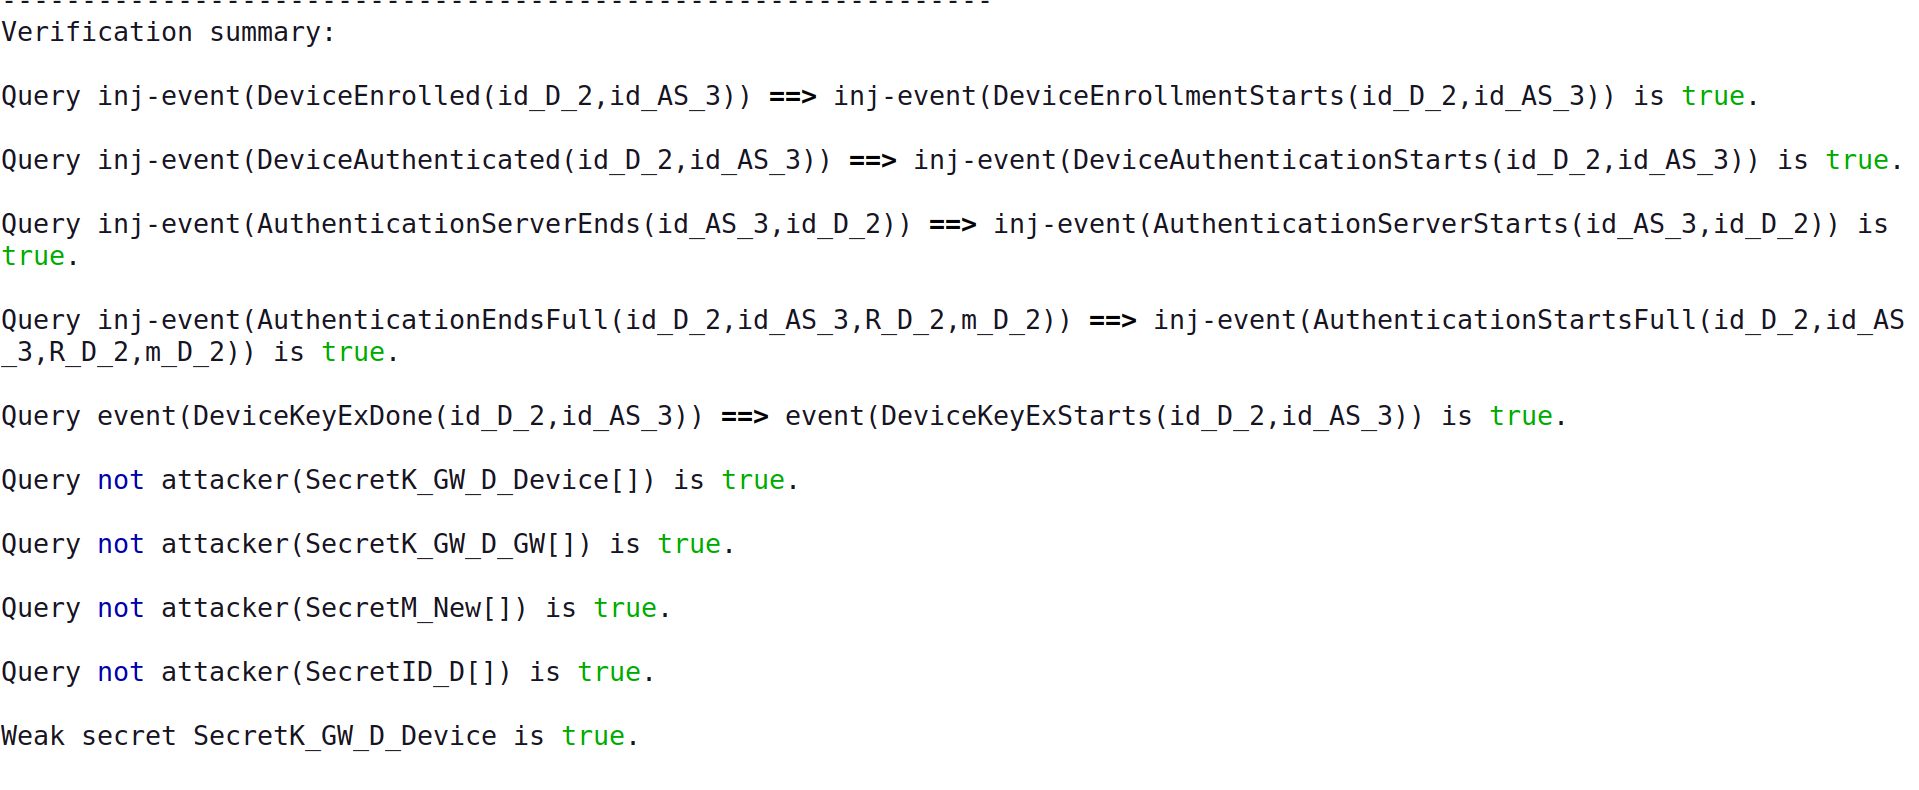
\includegraphics[width=\textwidth]{fig_proverif.png}
            {\scriptsize ProVerif verification output -- all queries return \texttt{true}.}
        \end{column}
    \end{columns}
\end{frame}

\begin{frame}{Informal Security Analysis}
    \footnotesize
    % 1 -- top left
    \noindent\begin{minipage}{0.54\textwidth}
        \begin{block}{Replay resistance}
            Timestamps ($ts_1,ts_2,ts_{\mathrm{auth}}$) + session random
            $m_{\mathrm{curr}}$ in every mask; stale messages fail freshness checks.
        \end{block}
    \end{minipage}\par
    \vspace{-0.15cm}
    % 2 -- mid right
    \noindent\hspace*{\fill}\begin{minipage}{0.54\textwidth}
        \begin{block}{MITM resistance}
            PUF response $R_D$ (unreproducible) and private $m_{\mathrm{curr}}$
            are embedded in every XOR mask -- no forgery possible.
        \end{block}
    \end{minipage}\par
    \vspace{-0.15cm}
    % 3 -- mid left
    \noindent\begin{minipage}{0.54\textwidth}
        \begin{block}{Device anonymity}
            $ID_D$ sent only once on the secure channel; open channel uses
            rotating, unlinkable $\mathit{PID}$.
        \end{block}
    \end{minipage}\par
    \vspace{-0.15cm}
    % 4 -- bottom right
    \noindent\hspace*{\fill}\begin{minipage}{0.54\textwidth}
        \begin{block}{Forward secrecy}
            $K_{GW\text{-}D}=H(R_D\|m_{\mathrm{new}})$; a compromised key reveals
            nothing about past/future keys.
        \end{block}
    \end{minipage}\par
\end{frame}

\begin{frame}{Theoretical Cost -- Enrolment Phase}
    \scriptsize
    \begin{center}
        \textbf{TABLE: Computational Cost Comparison: Enrolment Phase}
    \end{center}
    \vspace{-0.15cm}
    \begin{center}
        \renewcommand{\arraystretch}{1.15}
        \setlength{\tabcolsep}{4pt}
        \begin{tabular}{lll}
            \toprule
            Scheme & Operations & Cost (ms) \\
            \midrule
            LAAKA      & $3T_\mathsf{hash}$ & 0.11 \\
            Zhou et al. & $T_\mathsf{puf}+2T_\mathsf{hash}+3T_\mathsf{rand}$ & 0.13 \\
            DAuth      & $2T_\mathsf{puf}+1T_\mathsf{hash}+4T_\mathsf{rand}$ & 0.15 \\
            \textbf{Proposed} & $2T_\mathsf{puf}+2T_\mathsf{hash}+4T_\mathsf{rand}$ & \textbf{0.18} \\
            \bottomrule
        \end{tabular}
    \end{center}
    \vspace{-0.05cm}
    \begin{center}
        {\tiny Benchmark (avg.\ 100 iterations): $T_\mathsf{rand}$=0.0018\,ms, $T_\mathsf{puf}$=0.0522\,ms,
        $T_\mathsf{hash}$=0.0353\,ms, $T_\mathsf{aes}$=0.0867\,ms.}
    \end{center}

    \vspace{0.15cm}
    \begin{center}
        \textbf{TABLE: Communication Cost Comparison: Enrolment Phase}
    \end{center}
    \vspace{-0.15cm}
    \begin{center}
        \renewcommand{\arraystretch}{1.15}
        \setlength{\tabcolsep}{6pt}
        \begin{tabular}{lcc}
            \toprule
            Scheme & \# Messages & Cost (bits) \\
            \midrule
            LAAKA      & 3 & 2592 \\
            Zhou et al. & 5 & 1344 \\
            DAuth      & 3 & 1312 \\
            \textbf{Proposed} & 3 & \textbf{1312} \\
            \bottomrule
        \end{tabular}
    \end{center}
    \vspace{-0.05cm}
    \begin{center}
        {\tiny IDs/timestamps = 32\,b; hashes/nonces/challenges/ciphertexts = 256\,b.}
    \end{center}
\end{frame}

\begin{frame}{Theoretical Cost -- Authentication \& Key Exchange Phase}
    \scriptsize
    \begin{center}
        \textbf{TABLE: Computational Cost Comparison: Authentication \& Key Exchange Phase}
    \end{center}
    \vspace{-0.15cm}
    \begin{center}
        \renewcommand{\arraystretch}{1.15}
        \setlength{\tabcolsep}{4pt}
        \begin{tabular}{lll}
            \toprule
            Scheme & Operations & Cost (ms) \\
            \midrule
            LAAKA      & $16T_\mathsf{hash}$ & 0.56 \\
            Zhou et al. & $15T_\mathsf{hash}$ & 0.53 \\
            DAuth    & $2T_\mathsf{puf}+8T_\mathsf{hash}+2T_\mathsf{aes}+1T_\mathsf{rand}$ & 0.56 \\
            \textbf{Proposed} & $2T_\mathsf{puf}+11T_\mathsf{hash}+2T_\mathsf{aes}+T_\mathsf{rand}$ & \textbf{0.67} \\
            \bottomrule
        \end{tabular}
    \end{center}
    \vspace{-0.05cm}
    \begin{center}
        {\tiny Benchmark (avg.\ 100 iterations): $T_\mathsf{rand}$=0.0018\,ms, $T_\mathsf{puf}$=0.0522\,ms,
        $T_\mathsf{hash}$=0.0353\,ms, $T_\mathsf{aes}$=0.0867\,ms.}
    \end{center}

    \vspace{0.15cm}
    \begin{center}
        \textbf{TABLE: Communication Cost Comparison: Auth.\ \& Key Exchange Phase}
    \end{center}
    \vspace{-0.15cm}
    \begin{center}
        \renewcommand{\arraystretch}{1.15}
        \setlength{\tabcolsep}{6pt}
        \begin{tabular}{lcc}
            \toprule
            Scheme & \# Messages & Cost (bits) \\
            \midrule
            LAAKA      & 3 & 2400 \\
            Zhou et al. & 4 & 2464 \\
            DAuth    & 3 & 928 \\
            \textbf{Proposed} & 3 & \textbf{1376} \\
            \bottomrule
        \end{tabular}
    \end{center}
    \vspace{-0.05cm}
    \begin{center}
        {\tiny IDs/timestamps = 32\,b; hashes/nonces/challenges/ciphertexts = 256\,b.}
    \end{center}
\end{frame}

\begin{frame}{Simulation -- Per-Device Cost (COOJA / Contiki-NG)}
    \begin{columns}
        \begin{column}{0.4\textwidth}
            \footnotesize
            \textbf{Setup:} 100-node network, RPL Lite, CSMA, CoAP; 20 devices, 2 AS active;
            10 random seeds.
            \vspace{0.3cm}
            \begin{block}{Result}
                Proposed vs.\ state-of-the-art (per device, all phases):
                \begin{itemize}
                    \item Energy: \textbf{42.8\%} lower than LAAKA, \textbf{32.4\%} lower than Zhou.
                    \item CPU time: \textbf{42.7\%} / \textbf{32.4\%} lower.
                \end{itemize}
                
            \end{block}
        \end{column}
        \begin{column}{0.6\textwidth}
            \centering
            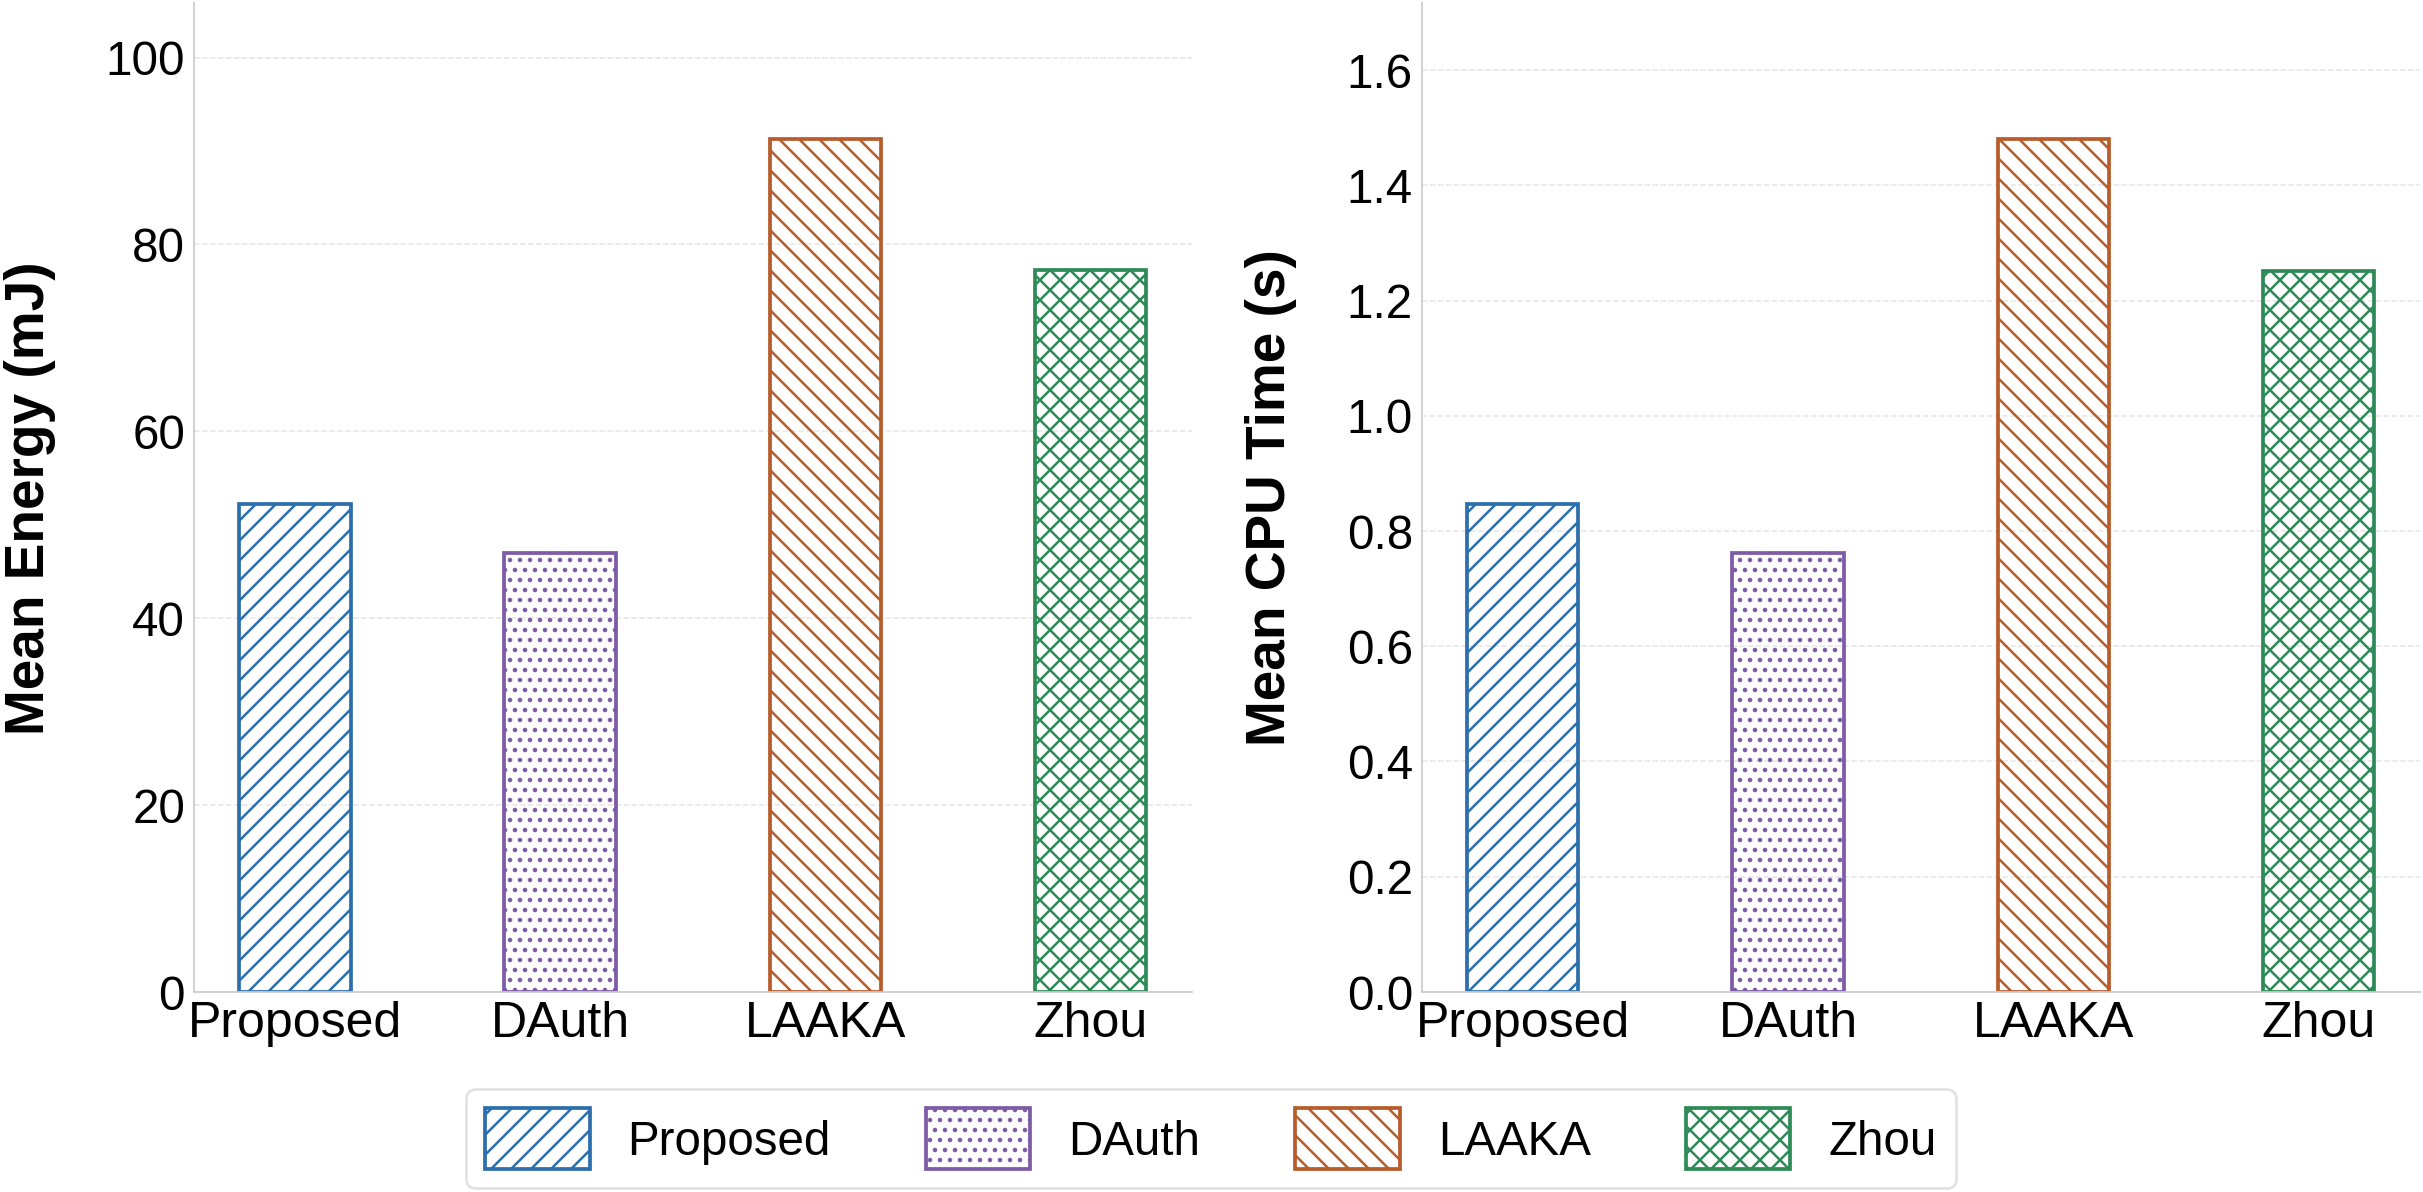
\includegraphics[width=\textwidth]{fig_sim_total.png}
            {\scriptsize (a) Energy \quad (b) CPU time -- mean per device.}
        \end{column}
    \end{columns}
\end{frame}

\begin{frame}{Simulation -- Authentication Server Pool Size}
    \begin{columns}
        \begin{column}{0.42\textwidth}
            \footnotesize
            AS pool grown from \textbf{2 to 10} servers (20 devices).
            \begin{itemize}
                \item Proposed stays $\sim$42\% below LAAKA at \emph{every} pool size.
                \item Both distributed schemes drop $\sim$11--12\% as the pool grows -- extra servers
                absorb join load.
                \item Zhou (gateway-coupled) is flat -- a centralised design \textbf{cannot} exploit
                AS diversity.
            \end{itemize}
        \end{column}
        \begin{column}{0.58\textwidth}
            \centering
            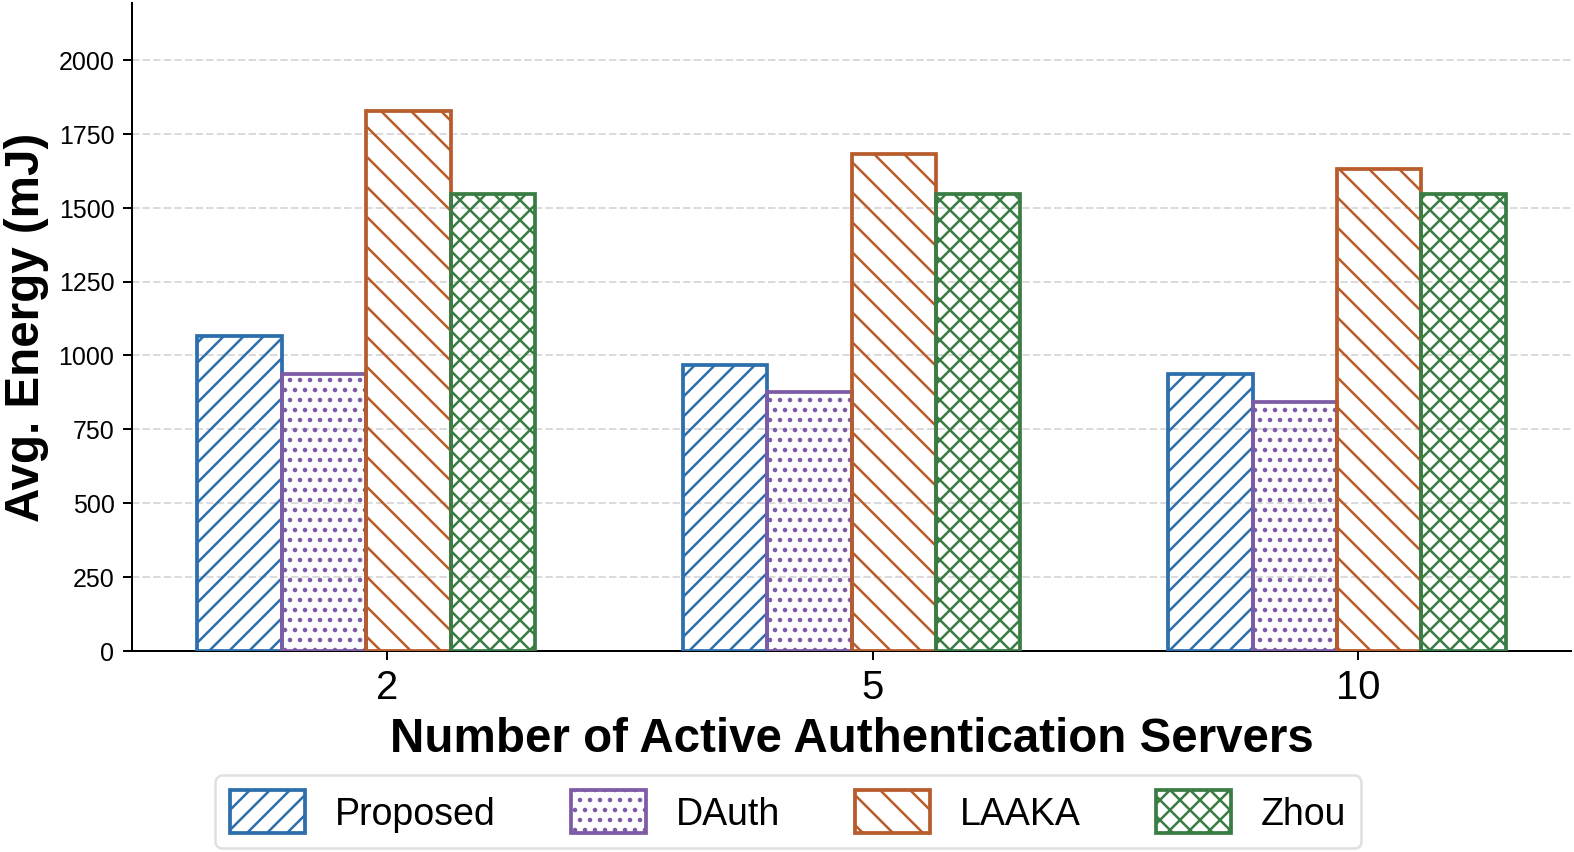
\includegraphics[width=0.78\textwidth]{fig_sim_as_energy.png}\\[-1pt]
            {\scriptsize (a) Total energy}\\[2pt]
            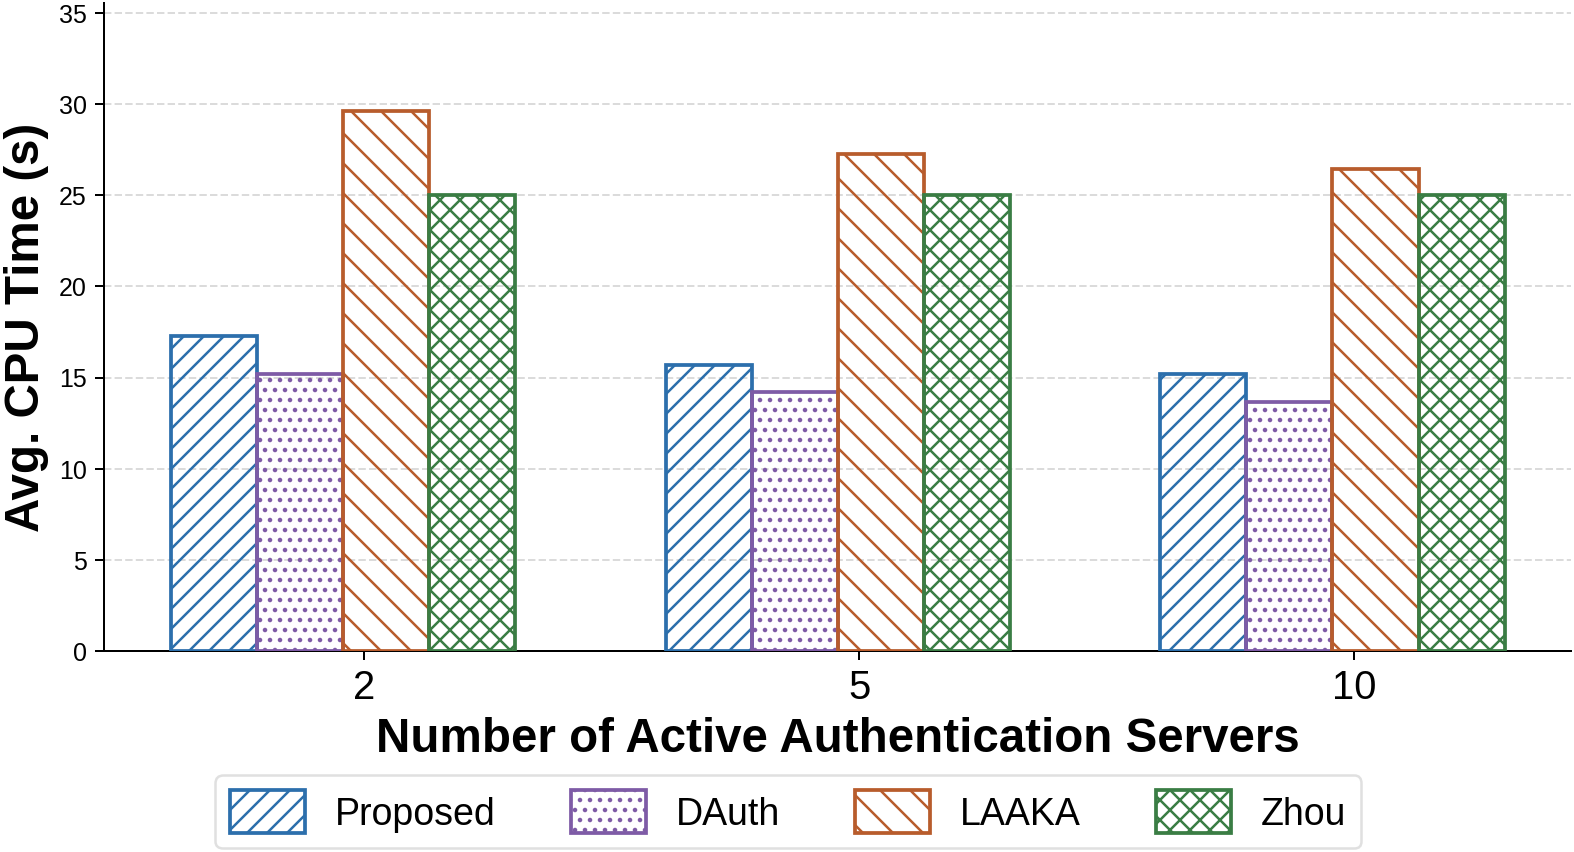
\includegraphics[width=0.78\textwidth]{fig_sim_as_cpu.png}\\[-1pt]
            {\scriptsize (b) Total CPU time}
        \end{column}
    \end{columns}
\end{frame}

\begin{frame}{Simulation -- Network Scalability}
    \begin{columns}
        \begin{column}{0.42\textwidth}
            \footnotesize
            Network size $N \in \{30,50,80,100,120\}$ (20\% newly-joined devices).
            \begin{itemize}
                \item At $N=120$: Proposed is \textbf{42.7\%} below LAAKA and \textbf{37.6\%} below Zhou
                in both energy and CPU time.
                \item LAAKA / Zhou grow steeply (AES-heavy crypto).
                \item Proposed stays lowest among anonymity-preserving schemes; only a small overhead above DAuth.
            \end{itemize}
        \end{column}
        \begin{column}{0.58\textwidth}
            \centering
            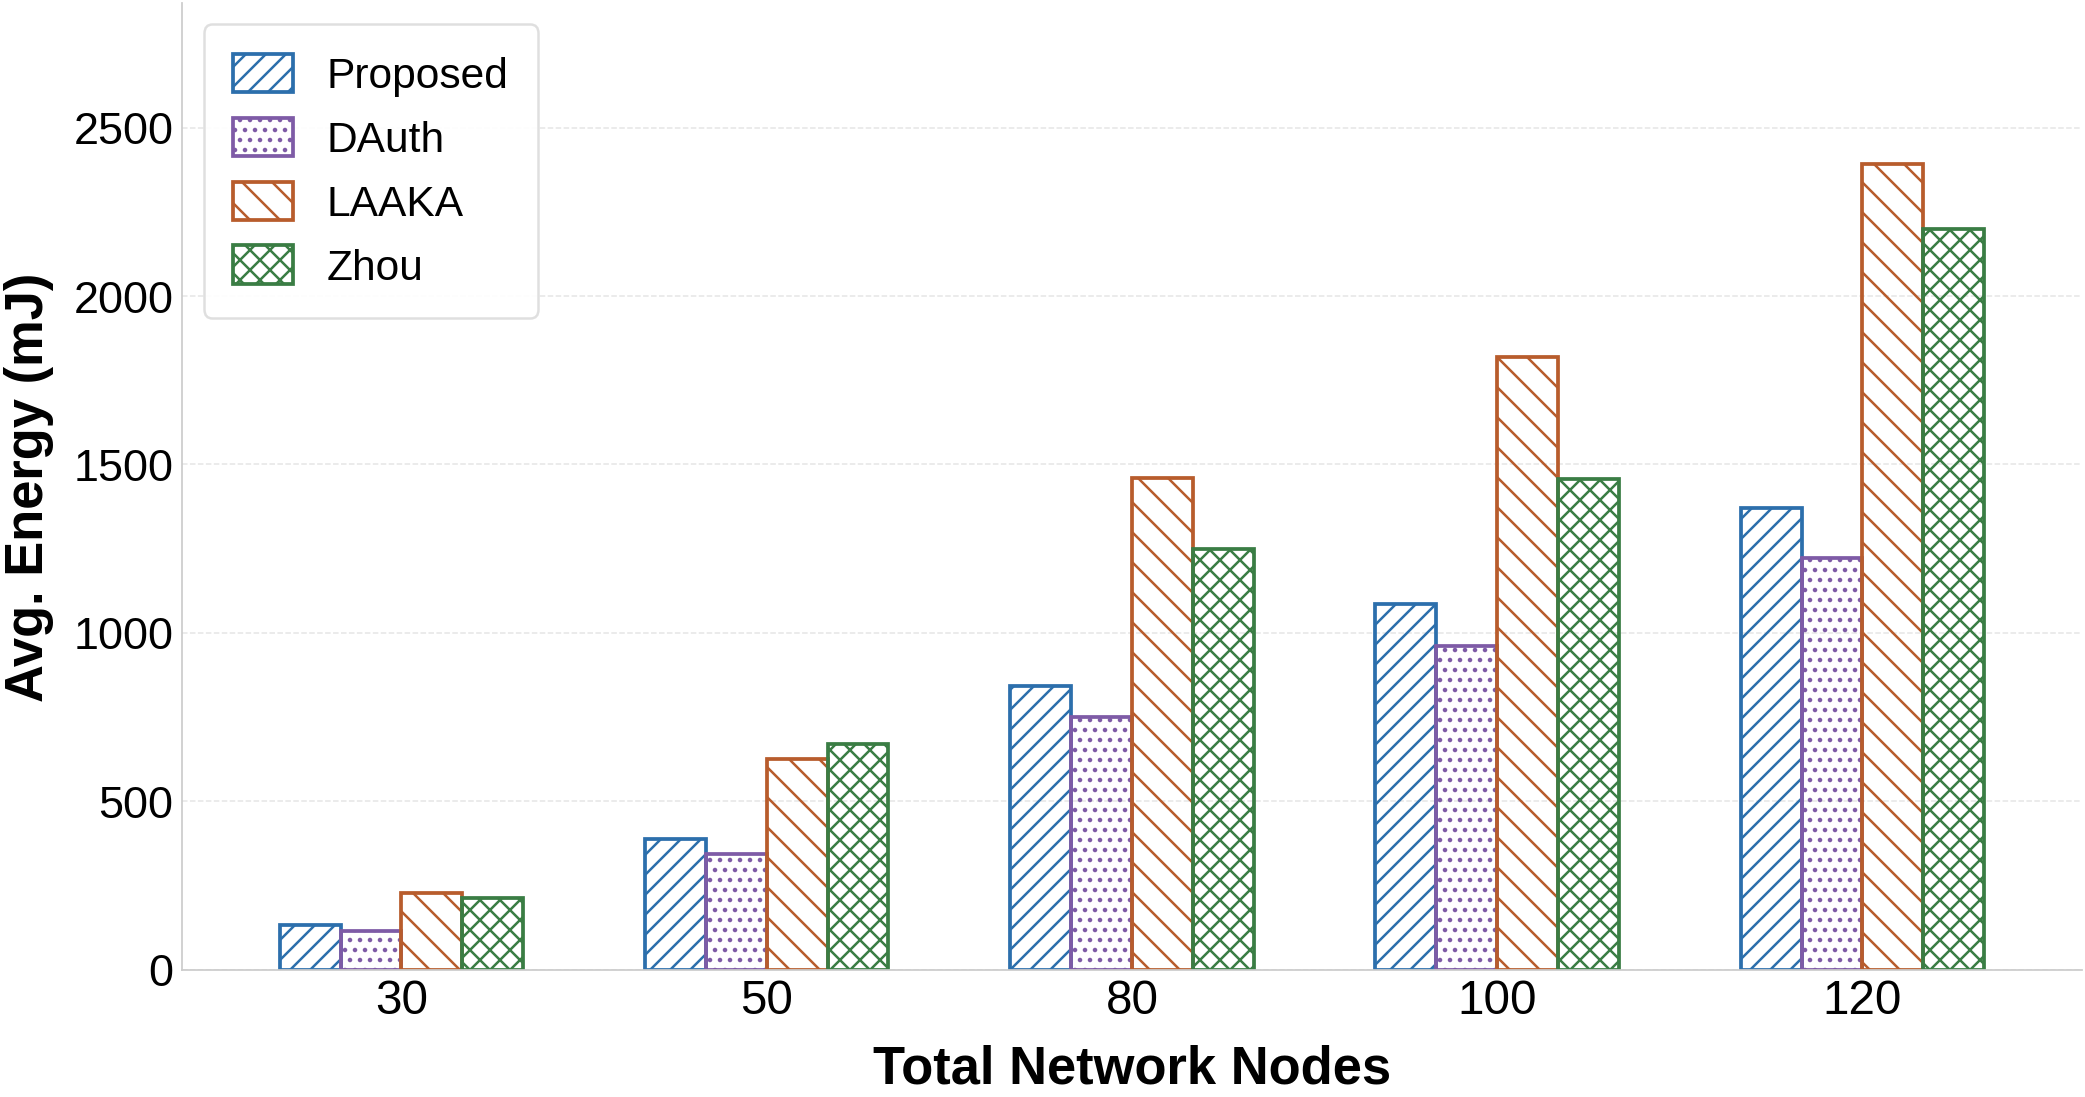
\includegraphics[width=0.78\textwidth]{fig_sim_net_energy.png}\\[-1pt]
            {\scriptsize (a) Total energy vs.\ $N$}\\[2pt]
            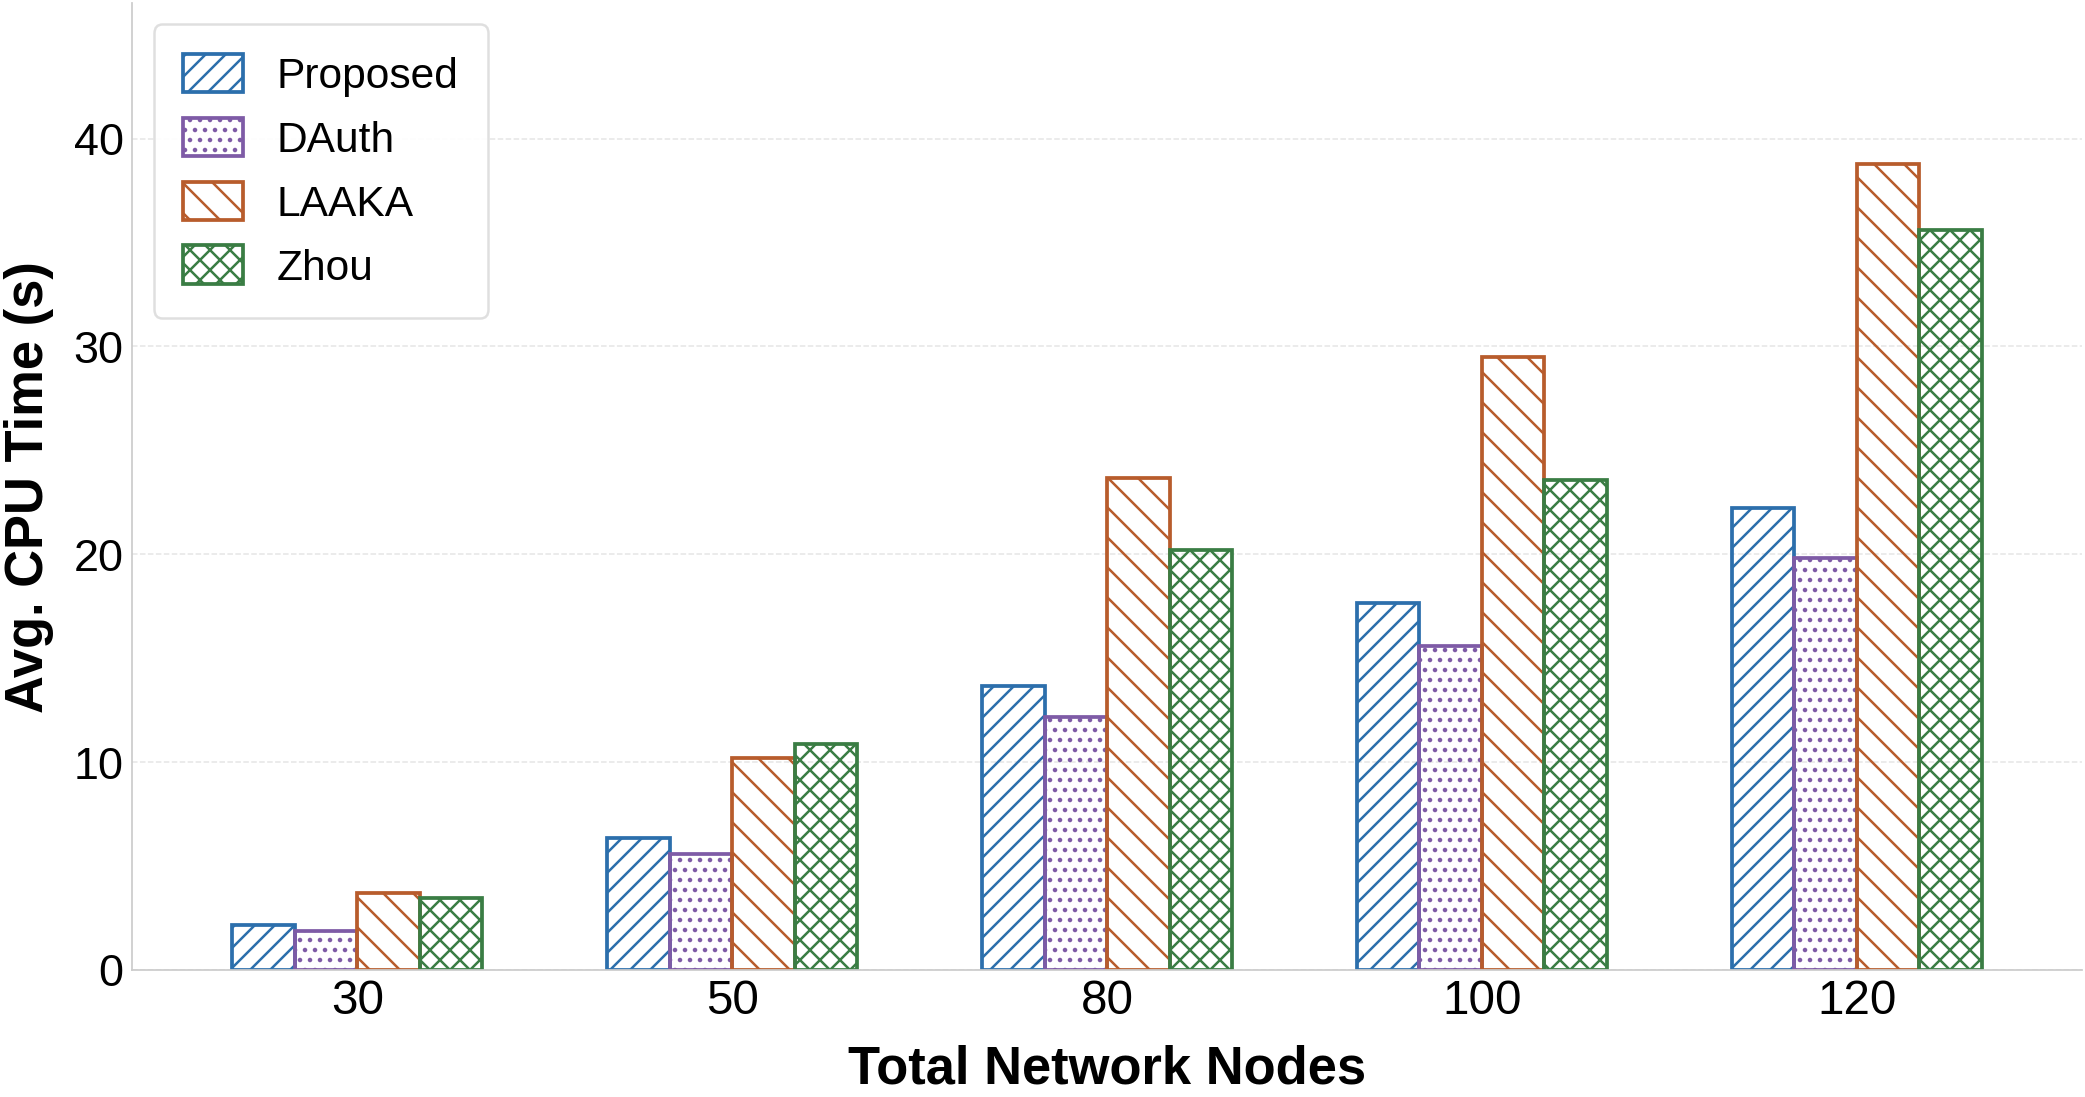
\includegraphics[width=0.78\textwidth]{fig_sim_net_cpu.png}\\[-1pt]
            {\scriptsize (b) Total CPU time vs.\ $N$}
        \end{column}
    \end{columns}
\end{frame}

\begin{frame}{Simulation -- Desynchronisation Recovery}
    \begin{columns}
        \begin{column}{0.42\textwidth}
            \footnotesize
            Per-device cost of one round: \textbf{normal} vs.\ \textbf{recovery} (round after a packet loss),
            100-node network, 20 devices, 5 seeds.
            \vspace{0.25cm}
            \begin{itemize}
                \item \textbf{DAuth}: recovery round costs \textbf{+118.3\%} energy (failed auth + full re-enrolment).
                \item \textbf{Proposed}: recovery $\approx$ normal -- dual state adds negligible overhead.
                \item Net: \textbf{35.3\%} lower recovery energy \emph{and} CPU time vs.\ DAuth.
            \end{itemize}
        \end{column}
        \begin{column}{0.58\textwidth}
            \centering
            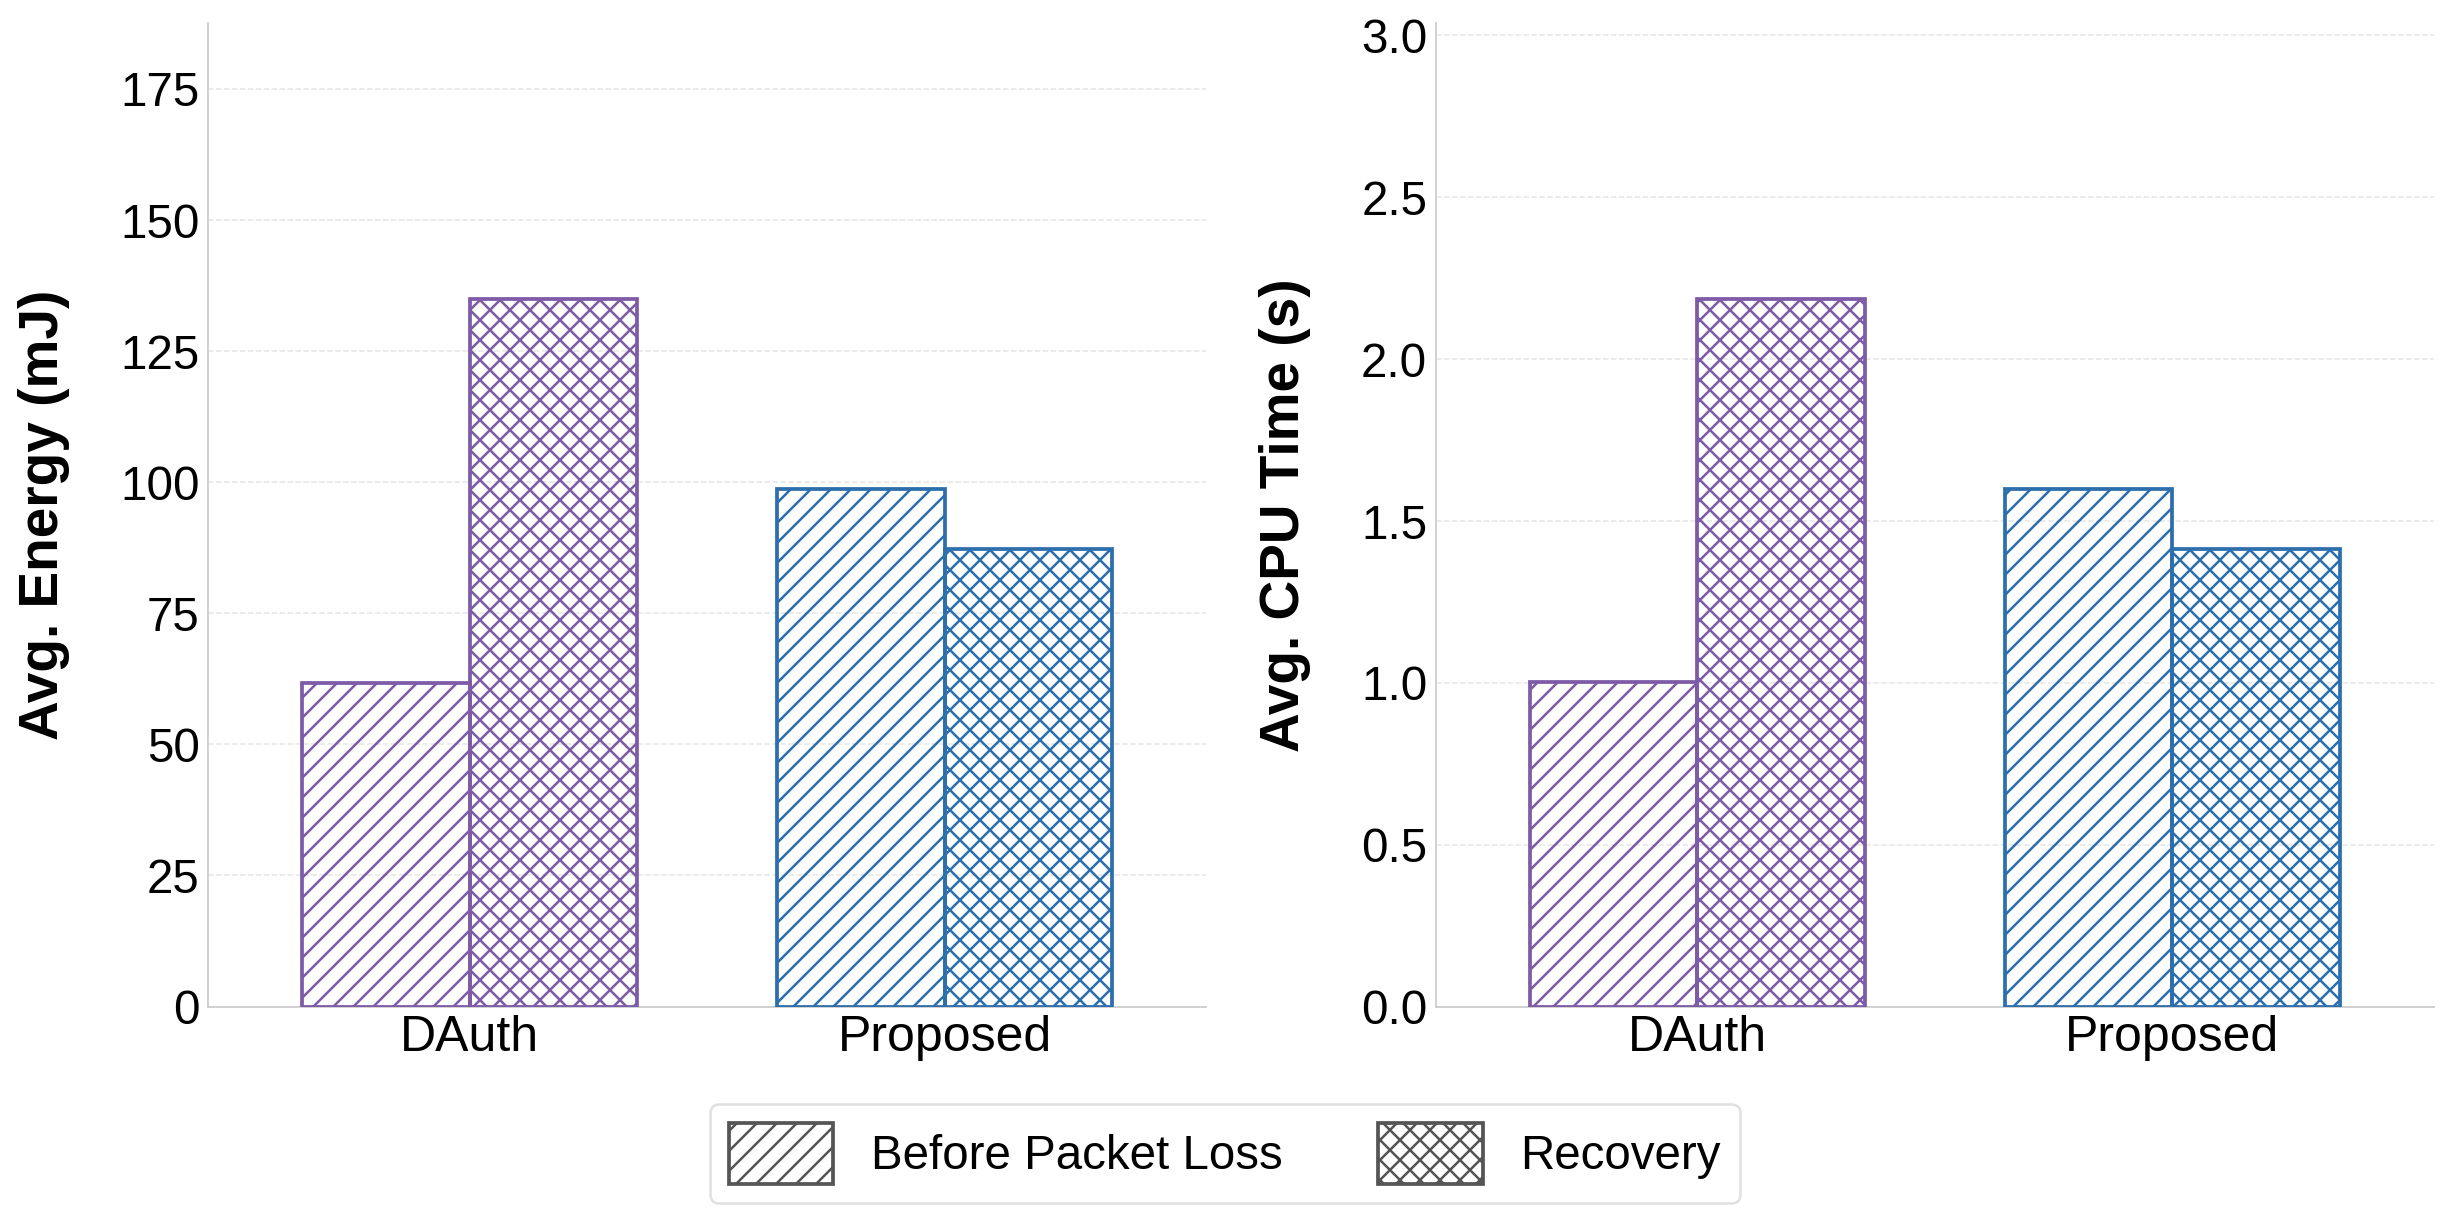
\includegraphics[width=\textwidth]{fig_desync_bar.png}
            {\scriptsize (a) Energy \quad (b) CPU time: normal vs.\ recovery round.}
        \end{column}
    \end{columns}
\end{frame}

\begin{frame}{Hardware Validation -- Raspberry Pi 4B Testbed}
    \begin{columns}
        \begin{column}{0.4\textwidth}
            \footnotesize
            \textbf{Setup:} 2$\times$ RPi 4B (device + AS), Windows laptop (GW), TCP links;
            energy $=$ wall-time $\times$ 3.8\,W.
            \vspace{0.25cm}
            \begin{block}{Per-round result}
                \begin{itemize}
                    \item Energy: Proposed 0.286\,J -- \textbf{14.2\%} below Zhou, \textbf{52.5\%} below LAAKA.
                    \item CPU: Proposed 0.075\,s -- \textbf{14.8\%} / \textbf{52.8\%} below Zhou / LAAKA.
                \end{itemize}
            \end{block}
        \end{column}
        \begin{column}{0.6\textwidth}
            \centering
            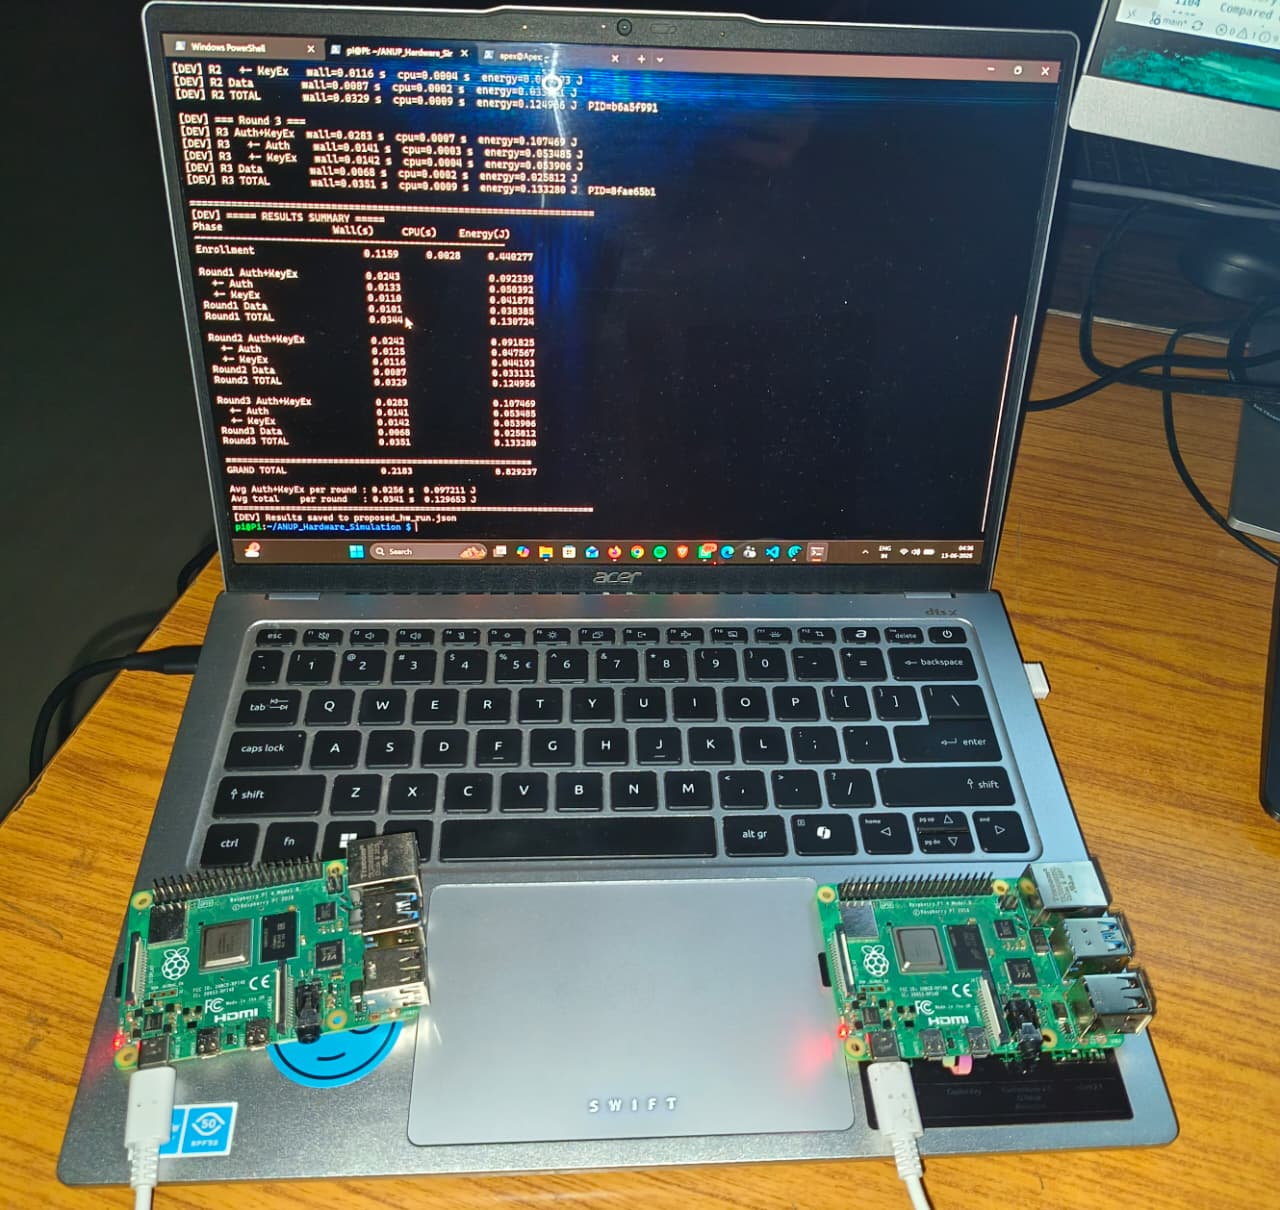
\includegraphics[width=0.58\textwidth]{fig_rpi_hw.jpeg}\\[2pt]
            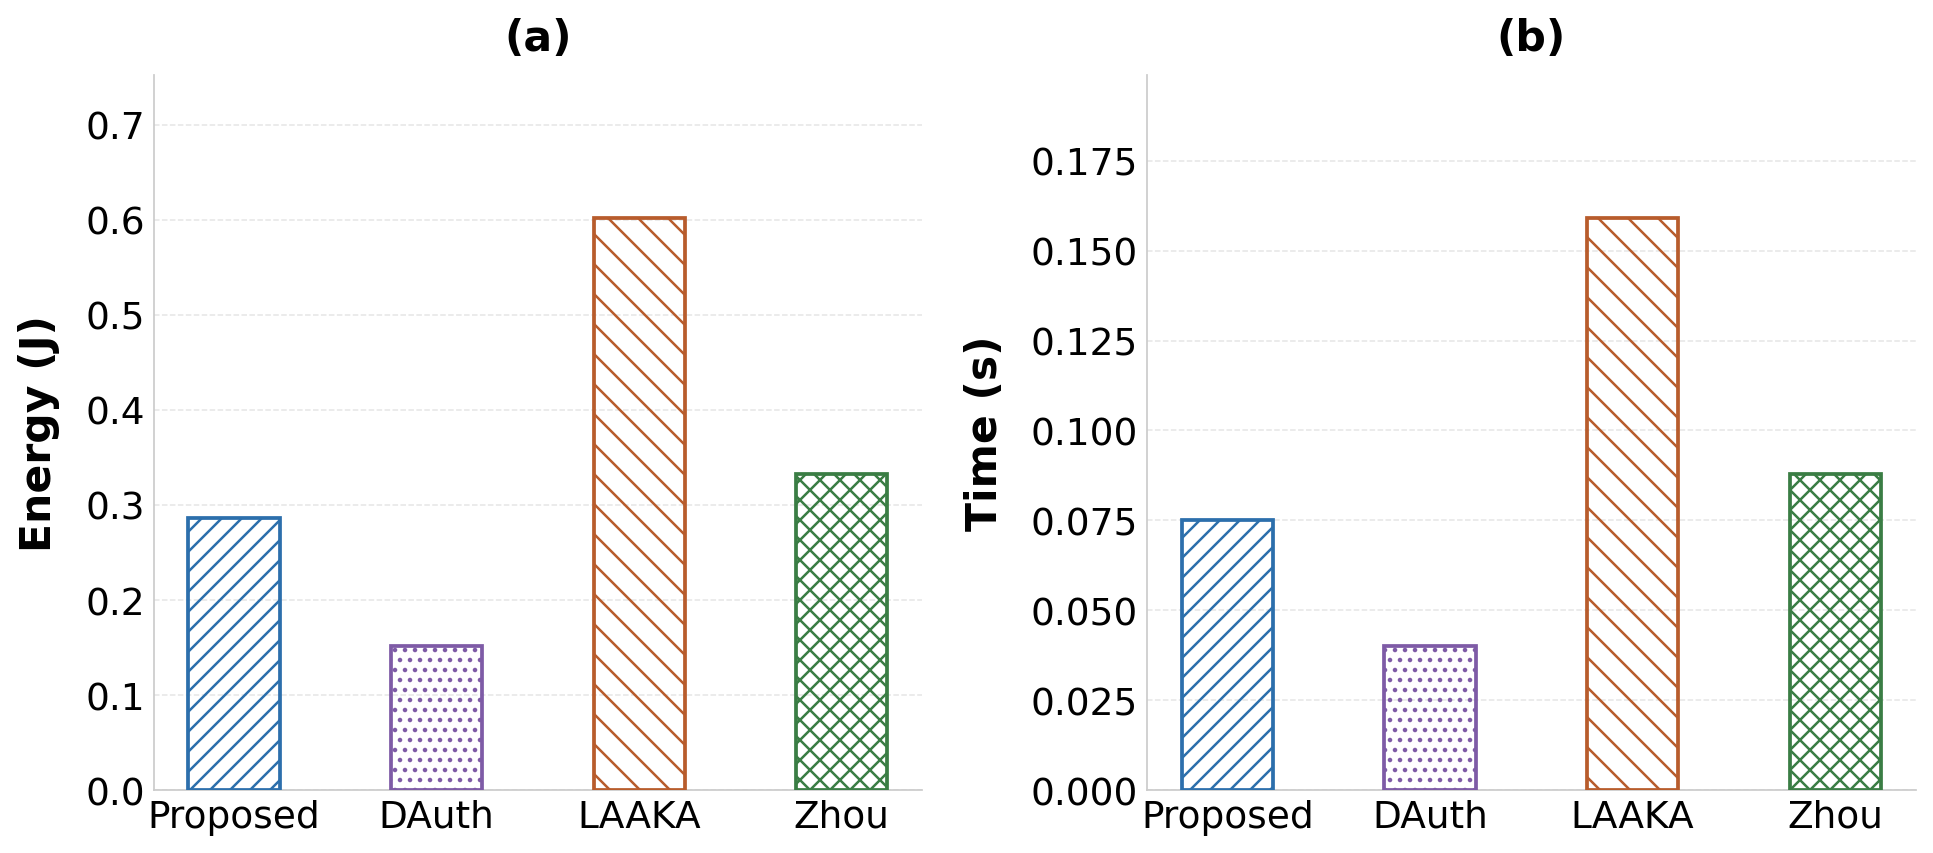
\includegraphics[width=0.92\textwidth]{fig_hw_comparison.png}\\[-1pt]
            {\scriptsize (a) Energy \quad (b) CPU time on RPi 4B.}
        \end{column}
    \end{columns}
\end{frame}
